\documentclass[11pt,a4paper]{article}
    \usepackage[margin=2.5cm]{geometry}
    \usepackage{enumitem}
    \usepackage{hyperref}
    \usepackage{tikz}
    \usetikzlibrary{arrows.meta,positioning,shapes.geometric}
    \title{Genome and Sequence Utilities}
    \author{CBBL Tools}
    \date{\today}

    \tikzset{
      methodbox/.style={
        rounded corners=6pt,
        draw=blue!50!black,
        line width=0.9pt,
        fill=blue!6,
        minimum width=13cm,
        text width=11.8cm,
        align=left,
        inner sep=8pt
      }
    }

    \begin{document}
    \maketitle

    \section*{Scope}
    This folder contains notebooks and scripts for retrieving biological sequences, parsing genome-related databases, and performing simple sequence transformations.

    \section*{Material in this folder}
    \begin{itemize}[leftmargin=*]
\item \texttt{RetrieveSequence.ipynb}
\item \texttt{apiUniprot.ipynb}
\item \texttt{parsinggnomAD.ipynb}
\item \texttt{parsinggnomAD.py}
\item \texttt{traduirSeqDNAaProt.ipynb}
    \end{itemize}

    \section*{Method summary}
    \begin{itemize}[leftmargin=*]
\item \textbf{Remote sequence retrieval}. The notebooks query external services such as UniProt to retrieve protein sequences and related records.
\item \textbf{gnomAD parsing}. The parsing material extracts and restructures information from genome variation resources.
\item \textbf{DNA to protein translation}. The translation notebook converts coding DNA strings to amino-acid sequences using the standard genetic code.
\item \textbf{Sequence-processing teaching examples}. The folder emphasizes small, readable examples for common bioinformatics tasks.
    \end{itemize}

    \section*{Method scheme}
    Figure~\ref{fig:summary} is drawn directly in LaTeX with TikZ. It is a compact conceptual map of the main workflows discussed in this folder.

    \begin{figure}[ht]
    \centering
    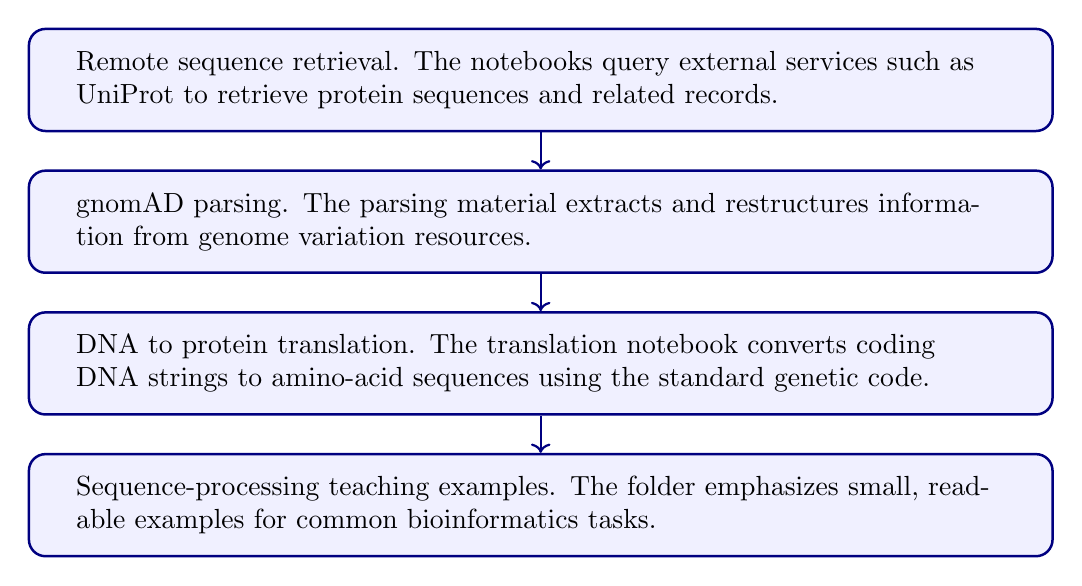
\begin{tikzpicture}[x=1cm,y=1cm]
    \node[methodbox] (m0) at (0,0.0) {Remote sequence retrieval. The notebooks query external services such as UniProt to retrieve protein sequences and related records.};
    \node[methodbox] (m1) at (0,-1.8) {gnomAD parsing. The parsing material extracts and restructures information from genome variation resources.};
    \node[methodbox] (m2) at (0,-3.6) {DNA to protein translation. The translation notebook converts coding DNA strings to amino-acid sequences using the standard genetic code.};
    \node[methodbox] (m3) at (0,-5.4) {Sequence-processing teaching examples. The folder emphasizes small, readable examples for common bioinformatics tasks.};
    \draw[->, thick, color=blue!50!black] (m0.south) -- (m1.north);
    \draw[->, thick, color=blue!50!black] (m1.south) -- (m2.north);
    \draw[->, thick, color=blue!50!black] (m2.south) -- (m3.north);
    \end{tikzpicture}
    \caption{Conceptual scheme for the methods in the genomeTools folder.}
    \label{fig:summary}
    \end{figure}

    \end{document}
